\documentclass{article}

\usepackage[spanish]{babel}
\usepackage[margin=1.5in]{geometry}
\usepackage{graphicx}
\usepackage[utf8]{inputenc}

\begin{document}

\setcounter{section}{-1}
\section{Conceptos básicos de redes eléctricas}

\subsection{Magnitudes eléctricas}

\begin{itemize}
	\item Intensidad de corriente eléctrica: Cantidad de carga que atraviesa un conductor por unidad de tiempo. Unidad: Ampère / Amperio (A). Órdenes usuales de magnitud (O.U.M.): $\mu$A, mA
	\item Diferencia de potencial (entre dos puntos): Causa/origen del paso de una corriente eléctrica a través
	de un conductor. Unidad: Volt/Voltio (V). O.U.M.: mV, V
	\item Frecuencia: Esta magnitud se verá más en detalle al ver corriente alterna. Unidad: Hertz (Hz).
	 O.U.M.: Hz, kHz, MHz.
\end{itemize}

\subsection{Tipos de señales}

Corriente Continua (CC) y Corriente Alterna (CA). En CC, la señal eléctrica se mantiene fija en un valor constante.
En CA, la señal varía de forma senoidal, con cierta amplitud, frecuencia y fase. Cuando estas señales son
generadas por fuentes, se usa la notación de la figura ~\ref{fig:fuentes}, en la página \pageref{fig:fuentes}

\begin{figure}[t]
\caption{Notación circuital para distintos tipos de fuentes}
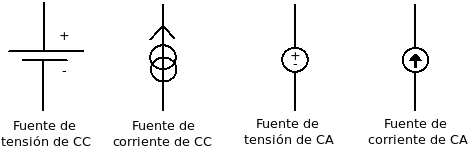
\includegraphics[scale=0.75]{img/teo_fig001_fuentes.png} 
\centering
\label{fig:fuentes}
\end{figure}

\end{document} 